%%%%%%%%%%%%%%%%%%%%%%%%%%%%%%%%%%%%%%%%%
% Lachaise Assignment
% LaTeX Template
% Version 1.0 (26/6/2018)
%
% This template originates from:
% http://www.LaTeXTemplates.com
%
% Authors:
% Marion Lachaise & François Févotte
% Vel (vel@LaTeXTemplates.com)
%
% License:
% CC BY-NC-SA 3.0 (http://creativecommons.org/licenses/by-nc-sa/3.0/)
% 
%%%%%%%%%%%%%%%%%%%%%%%%%%%%%%%%%%%%%%%%%

%----------------------------------------------------------------------------------------
%	PACKAGES AND OTHER DOCUMENT CONFIGURATIONS
%----------------------------------------------------------------------------------------

\documentclass{article}
\usepackage{amsthm}
\usepackage{listings}
\usepackage{xcolor}
\usepackage{graphicx}


\lstset{
	language=Python,
	basicstyle=\ttfamily\small,
	keywordstyle=\color{blue},
	stringstyle=\color{red},
	commentstyle=\color{purple},
	showstringspaces=false,
	numbers=left,
	numberstyle=\tiny\color{gray},
	breaklines=true,
	frame=single,
	captionpos=b
}
\newtheorem{definition}{Definition}[section]
\newtheorem{proposition}{Proposition}
\newtheorem{corolary}{Corolary}

%%%%%%%%%%%%%%%%%%%%%%%%%%%%%%%%%%%%%%%%%
% Lachaise Assignment
% Structure Specification File
% Version 1.0 (26/6/2018)
%
% This template originates from:
% http://www.LaTeXTemplates.com
%
% Authors:
% Marion Lachaise & François Févotte
% Vel (vel@LaTeXTemplates.com)
%
% License:
% CC BY-NC-SA 3.0 (http://creativecommons.org/licenses/by-nc-sa/3.0/)
% 
%%%%%%%%%%%%%%%%%%%%%%%%%%%%%%%%%%%%%%%%%

%----------------------------------------------------------------------------------------
%	PACKAGES AND OTHER DOCUMENT CONFIGURATIONS
%----------------------------------------------------------------------------------------

\usepackage{amsmath,amsfonts,stmaryrd,amssymb} % Math packages

\usepackage{enumerate} % Custom item numbers for enumerations

\usepackage[ruled]{algorithm2e} % Algorithms

\usepackage[framemethod=tikz]{mdframed} % Allows defining custom boxed/framed environments

\usepackage{listings} % File listings, with syntax highlighting
\lstset{
	basicstyle=\ttfamily, % Typeset listings in monospace font
}

%----------------------------------------------------------------------------------------
%	DOCUMENT MARGINS
%----------------------------------------------------------------------------------------

\usepackage{geometry} % Required for adjusting page dimensions and margins

\geometry{
	paper=a4paper, % Paper size, change to letterpaper for US letter size
	top=2.5cm, % Top margin
	bottom=3cm, % Bottom margin
	left=2.5cm, % Left margin
	right=2.5cm, % Right margin
	headheight=14pt, % Header height
	footskip=1.5cm, % Space from the bottom margin to the baseline of the footer
	headsep=1.2cm, % Space from the top margin to the baseline of the header
	%showframe, % Uncomment to show how the type block is set on the page
}

%----------------------------------------------------------------------------------------
%	FONTS
%----------------------------------------------------------------------------------------

\usepackage[utf8]{inputenc} % Required for inputting international characters
\usepackage[T1]{fontenc} % Output font encoding for international characters

\usepackage{XCharter} % Use the XCharter fonts

%----------------------------------------------------------------------------------------
%	COMMAND LINE ENVIRONMENT
%----------------------------------------------------------------------------------------

% Usage:
% \begin{commandline}
%	\begin{verbatim}
%		$ ls
%		
%		Applications	Desktop	...
%	\end{verbatim}
% \end{commandline}

\mdfdefinestyle{commandline}{
	leftmargin=10pt,
	rightmargin=10pt,
	innerleftmargin=15pt,
	middlelinecolor=black!50!white,
	middlelinewidth=2pt,
	frametitlerule=false,
	backgroundcolor=black!5!white,
	frametitle={Command Line},
	frametitlefont={\normalfont\sffamily\color{white}\hspace{-1em}},
	frametitlebackgroundcolor=black!50!white,
	nobreak,
}

% Define a custom environment for command-line snapshots
\newenvironment{commandline}{
	\medskip
	\begin{mdframed}[style=commandline]
}{
	\end{mdframed}
	\medskip
}

%----------------------------------------------------------------------------------------
%	FILE CONTENTS ENVIRONMENT
%----------------------------------------------------------------------------------------

% Usage:
% \begin{file}[optional filename, defaults to "File"]
%	File contents, for example, with a listings environment
% \end{file}

\mdfdefinestyle{file}{
	innertopmargin=1.6\baselineskip,
	innerbottommargin=0.8\baselineskip,
	topline=false, bottomline=false,
	leftline=false, rightline=false,
	leftmargin=2cm,
	rightmargin=2cm,
	singleextra={%
		\draw[fill=black!10!white](P)++(0,-1.2em)rectangle(P-|O);
		\node[anchor=north west]
		at(P-|O){\ttfamily\mdfilename};
		%
		\def\l{3em}
		\draw(O-|P)++(-\l,0)--++(\l,\l)--(P)--(P-|O)--(O)--cycle;
		\draw(O-|P)++(-\l,0)--++(0,\l)--++(\l,0);
	},
	nobreak,
}

% Define a custom environment for file contents
\newenvironment{file}[1][File]{ % Set the default filename to "File"
	\medskip
	\newcommand{\mdfilename}{#1}
	\begin{mdframed}[style=file]
}{
	\end{mdframed}
	\medskip
}

%----------------------------------------------------------------------------------------
%	NUMBERED QUESTIONS ENVIRONMENT
%----------------------------------------------------------------------------------------

% Usage:
% \begin{question}[optional title]
%	Question contents
% \end{question}

\mdfdefinestyle{question}{
	innertopmargin=1.2\baselineskip,
	innerbottommargin=0.8\baselineskip,
	roundcorner=5pt,
	nobreak,
	singleextra={%
		\draw(P-|O)node[xshift=1em,anchor=west,fill=white,draw,rounded corners=5pt]{%
		Question \theQuestion\questionTitle};
	},
}

\newcounter{Question} % Stores the current question number that gets iterated with each new question

% Define a custom environment for numbered questions
\newenvironment{question}[1][\unskip]{
	\bigskip
	\stepcounter{Question}
	\newcommand{\questionTitle}{~#1}
	\begin{mdframed}[style=question]
}{
	\end{mdframed}
	\medskip
}

%----------------------------------------------------------------------------------------
%	WARNING TEXT ENVIRONMENT
%----------------------------------------------------------------------------------------

% Usage:
% \begin{warn}[optional title, defaults to "Warning:"]
%	Contents
% \end{warn}

\mdfdefinestyle{warning}{
	topline=false, bottomline=false,
	leftline=false, rightline=false,
	nobreak,
	singleextra={%
		\draw(P-|O)++(-0.5em,0)node(tmp1){};
		\draw(P-|O)++(0.5em,0)node(tmp2){};
		\fill[black,rotate around={45:(P-|O)}](tmp1)rectangle(tmp2);
		\node at(P-|O){\color{white}\scriptsize\bf !};
		\draw[very thick](P-|O)++(0,-1em)--(O);%--(O-|P);
	}
}

% Define a custom environment for warning text
\newenvironment{warn}[1][Warning:]{ % Set the default warning to "Warning:"
	\medskip
	\begin{mdframed}[style=warning]
		\noindent{\textbf{#1}}
}{
	\end{mdframed}
}

%----------------------------------------------------------------------------------------
%	INFORMATION ENVIRONMENT
%----------------------------------------------------------------------------------------

% Usage:
% \begin{info}[optional title, defaults to "Info:"]
% 	contents
% 	\end{info}

\mdfdefinestyle{info}{%
	topline=false, bottomline=false,
	leftline=false, rightline=false,
	nobreak,
	singleextra={%
		\fill[black](P-|O)circle[radius=0.4em];
		\node at(P-|O){\color{white}\scriptsize\bf i};
		\draw[very thick](P-|O)++(0,-0.8em)--(O);%--(O-|P);
	}
}

% Define a custom environment for information
\newenvironment{info}[1][Info:]{ % Set the default title to "Info:"
	\medskip
	\begin{mdframed}[style=info]
		\noindent{\textbf{#1}}
}{
	\end{mdframed}
}
 % Include the file specifying the document structure and custom commands

%----------------------------------------------------------------------------------------
%	ASSIGNMENT INFORMATION
%----------------------------------------------------------------------------------------

\title{LISTA 2 DE MAC5770 - EMPARELHAMENTOS EM GRAFOS} % Title of the assignment

\author{Giovani Tavares (10788620)\\ \texttt{giovanitavares@usp.br}} % Author name and email address

\date{University of Sao Paulo --- 2025.1} % University, school and/or department name(s) and a date

%----------------------------------------------------------------------------------------

\begin{document}

\maketitle % Print the title

%----------------------------------------------------------------------------------------
%	INTRODUCTION
%----------------------------------------------------------------------------------------

\section{20 de Maio, 2025} % Unnumbered section


 \subsection{Exercício 1:  Seja $G$ um grafo simples de ordem $n$, $n$ par. Prove que se $d(v) > n/2$ para todo $v \in V (G)$, então $G$ contém $3$ emparelhamentos perfeitos dois a dois disjuntos.}
 
 \section*{Parte I}
 
 Mostrando que todo ciclo hamiltoniano pode ser escrito como a união de dois emparelhamentos perfeitos disjuntos.
 
 Pelo Teorema de Dirac, se $d(v) > n/2$, então $G$ tem um ciclo hamiltoniano.
 
 Seja $H = (v_1, v_2, \ldots, v_n, v_1)$, um ciclo hamiltoniano de $G$.
 
 Podemos escrever o ciclo $H$ como um conjunto de arestas:
 
 $$
 H = \{ \{v_1, v_2\}, \{v_2, v_3\}, \ldots, \{v_{n-1}, v_n\}, \{v_n, v_1\} \}
 $$
 
 Ou seja, podemos escrever $H$ como a união de dois conjuntos disjuntos de arestas:
 
 $$
 H = \left[ \{ \{v_1, v_2\}, \{v_3, v_4\}, \{v_5, v_6\}, \ldots, \{v_{n-1}, v_n\} \} \right] \cup
 \left[ \{ \{v_2, v_3\}, \{v_4, v_5\}, \{v_6, v_7\}, \ldots, \{v_n, v_1\} \} \right]
 $$
 
 Ou seja, podemos escrever $H$ como a união de dois conjuntos disjuntos de arestas:
 
 $$
 A = \bigcup_{i \text{ ímpar}}^{n-1} \{ \{v_i, v_{i+1}\} \}, \quad 
 B = [\bigcup_{j \text{ par}}^{n-1} \{ \{v_j, v_{j+1}\} \}] \cup \{ \{v_n, v_1\} \}
 $$
 
 $A$ é emparelhamento perfeito, pois cobre os $n$ vértices de $G$ e não contém arestas adjacentes, o mesmo valendo para $B$. Além disso, $A$ e $B$ são disjuntos, pois uma aresta $\{v_i, v_{i+1}\}$ não pode ter $i$ par e ímpar simultaneamente (i.e., não pode estar em $A$ e $B$ ao mesmo tempo).
 
 Assim, o ciclo hamiltoniano $H$ pode ser escrito como a união de dois emparelhamentos perfeitos disjuntos. Como $H$ é arbitrário, pode-se concluir que todo ciclo hamiltoniano pode ser escrito como a união de dois emparelhamentos perfeitos disjuntos.
 
 \section*{Parte II}
 
 Mostrando que, se $G$ é tal que $v(G) = n$, $n$ par, e $d(v) > n/2$ para todo vértice $v$ de $G$, então $G$ tem 3 emparelhamentos perfeitos dois a dois disjuntos.
 
 Como $\forall v \in V(G)$, $d(v) > n/2$, então, pelo Teorema de Dirac, $G$ tem um ciclo hamiltoniano $H$. 
 
 Como demonstrado anteriormente na \textbf{Parte I}, $H$ pode ser escrito como a união de dois emparelhamentos perfeitos. Chamemos-nos de $M_1$ e $M_2$:
 
 $$
 H = M_1 \cup M_2
 $$
 
 Pode-se afirmar que $G$ tem 2 emparelhamentos perfeitos disjuntos.
 
 Seja $G' = G \setminus M_1$, o grafo formado pela retirada das arestas de $M_1$ de $G$.
 
 Como $M_1$ é emparelhamento perfeito, temos que $\forall v \in V(G), d_{M_1} = 1$, entao: 
 
 Portanto:
 
 $$
 d_{G'}(v) = d_G(v) - d_{M_1}  =  d_G(v) - 1
 $$
 
 Com $d_G(v) > n/2$ e $n$ par. Como $d_G(v) \in \mathbb{Z}$, temos:
 
 \begin{align*}
 	d_G(v) &> \frac{n}{2} \\
 	\implies d_{G}(v) &\geq \frac{n}{2}  + 1\\
    \implies d_G(v) - 1 &\geq (\frac{n}{2} + 1) - 1 \\
  	\implies d_{G'}(v) &\geq \frac{n}{2}
 \end{align*}
 
 Assim, pelo Teorema de Dirac, $G'$ também tem um ciclo hamiltoniano $H'$. Como demonstrado na \textbf{Parte I}, $H'$ pode ser escrito como a união de dois emparelhamentos perfeitos disjuntos $M_3$ e $M_4$:
 
 $$
 H' = M_3 \cup M_4
 $$
 
 Sabemos que $M_3$ e $M_4$ também são emparelhamentos perfeitos de $G$, pois $V(G) = V(G')$ e $E(G') \subset E(G)$.
 
 Além disso, $M_1 \cap M_3 = M_1 \cap M_4 = \varnothing$, pois as arestas de $M_1$ foram removidas para formar $G'$. 
 
 Assim, $M_1, M_3$ e $M_4$ são três emparelhamentos perfeitos dois a dois disjuntos de $G$ e, portanto, $G$ tem $3$ emparelhamentos perfeitos dois a dois disjuntos.
 
 \clearpage
 
 \subsection{Exercício 2:  Prove que toda árvore tem no máximo um emparelhamento perfeito. De um exemplo de uma árvore sem emparelhamento perfeito.}

Utilizemos uma prova por inducao.


  \subsubsection*{Caso Base}
  
  Seja $T$ uma árvore com dois vértices. O emparelhamento perfeito de $T$ contém a única aresta de $T$ e é único, pois nao existe apenas uma aresta incidente a seus dois únicos vértices.
  
  
  
  \subsubsection*{Hipótese de Inducao}
  
  Suponhamos que toda árvore $T$ com $k < n$ vértices seja tal que tenha no máximo um emparelhamento perfeito.
  
  Seja $T$ uma árvore com $n$ vértices, i.e., $v(T) = n$. Seja $M$ um emparelhamento perfeito de $T$.

 $T$ é árvore, entao $V(T)$ tem pelo menos um vértice $f$ que é folha, i.e., um vértice $f$ tal que $d_T(f) = 1$.
  
Como $d_T(f) = 1$, existe um vértice $u \neq f$, $u \in V(T)$, tal que $u$ é vizinho de $f$.
  
Seja $F$ a floresta formada pela retirada dos vértices $u$ e $f$ de $T$, i.e., 

\begin{align*}
	E(F) &=  E(T) \setminus  \{   \{u,f\}   \} \\
	V(F) &=  V(T) \setminus \{u,f\} \\
	&\implies v(F) = v(T) - 2 = n - 2 < n \\
	&\implies \text{F tem no máximo um emparelhamento perfeito, pela hipótese de inducao.}  \\
\end{align*}

Chamemos $M'$ o emparelhamento perfeito único de $F$. Como $F$ tem exatamente as mesmas arestas de $T$ com exececao da única incidente a $f$, chamada $\{u,f\}$, pode-se afirmar que a adicao da aresta $\{\{u,f\}\}$ a $M'$ recupera $M$, i.e. :

\begin{align}
	M = M' \cup \{\{u,f\}\}
\end{align}

Como $\{u,f\}$ é a única aresta incidente a $f$ na árvore $T$, pois $f$ é folha, $\{u,f\}$ é aresta presente em qualquer emparelhamento perfeito de $T$. Assim, para gerar emparelhamento perfeito de $T$ distinto de $M$, é preciso substituir pelo menos uma aresta $e'$ de $M'$ por alguma aresta $e_{sub} \in E(T)$ nao presente entre as arestas de $M'$, formando o conjunto de arestas $M''$.  $e_{sub} \neq \{u,v\}$, pois $e_{sub}$ deve ser incidente a pelo menos um dos vértices aos quais incide $e'$, e os vértices $u$ e $f$ nao estao entre os vértices das arestas de $M'$.

 $M'$ é emparelhamento perfeito único da floresta $F$ por hipótese, o que indica que nao existe nenhum outro conjunto de arestas nao adjascentes que cubram todos os vértices de $F$, i.e., $M''$ nao é emparelhamento. Assim, 


\begin{align}
	M = M'' \cup \{\{u,f\}\}
\end{align}

é uma contradicao, pois $M$ nao pode ser um emparelhamento perfeito com um subconjunto de arestas $M''$ que nao é um emparelhamento. 

Assim, o emparelhamento $M$ é único e tal que

\begin{align}
	M = M' \cup \{\{u,f\}\}
\end{align}

Estando demonstrado que vale a afirmacao vale para árvores $T$ tais que $v(T) = n$


 \subsubsection*{Exemplo de árvore sem emparelhamento perfeito}

 A árvore definida por 
 
 \begin{align*}
 	E(T) &=  \{\{u_1,u_2\},\{u_2,u_3\}    \} \\
 	V(T) &=  \{u_1,u_2,u_3\}
 \end{align*}
 
  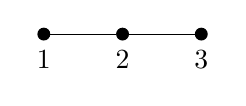
\begin{tikzpicture}
 	% Define the vertices
 	\node[circle, draw, fill=black, inner sep=1.5pt, label=below:1] (v1) at (0,0) {};
 	\node[circle, draw, fill=black, inner sep=1.5pt, label=below:2] (v2) at (1,0) {};
 	\node[circle, draw, fill=black, inner sep=1.5pt, label=below:3] (v3) at (2,0) {};
 	
 	% Draw the edges
 	\draw (v1) -- (v2);
 	\draw (v2) -- (v3);
 \end{tikzpicture}
 
 Nao tem emparelhamento perfeito, pois tem um número ímpar de vértices.
\clearpage


 \subsection{Exercício 3:  Seja $G$ um grafo $(X, Y)-\text{bipartido}$ simples tal que $|X| = |Y | = n \geq 1$. Prove que se $e(G) > n(n - 1)$ então $G$ tem um emparelhamento perfeito.}
 
 Suponhamos, por absurdo, que $G$ não tem um emparelhamento perfeito. Então, pelo Teorema de Hall, $\exists S \subseteq X$ tal que $|N(S)| < |S|$. Seja $|S| = s$.
 
 O objetivo é chegar em uma contradição e encontrar um limite superior para $e(G)$ sob a suposição. Pode-se afirmar:
 
 $$1 \leq s \leq n - 1,$$ pois $s = |S|$ e $S \subset X$.  
 $$|N(S)| < s$$ por suposição.
 
 Cada vértice de $S$ está conectado a somente vértices em $N(S)$. Assim, o número máximo de arestas entre $S$ e $N(S)$ é igual ao produto de $s$ com $|N(S)|$, i.e.,
 
 $$\sum_{u \in S} d(u) \leq |S| \cdot |N(S)| = s \cdot |N(S)|$$  
 que corresponde ao número máximo de arestas adjascentes aos vértices de $S$, pois $S \subseteq X$ e $G$ é $(X, Y)-\text{bipartido}$.
 
 Cada vértice de $X \setminus S$ pode estar conectado a qualquer vértice de $Y$, exceto aos vértices de $Y$ conectados a $S$ (i.e., exceto aos vértices de $N(S)$).
 
 Assim, o número máximo de arestas de $X \setminus S$ para $Y$ é:
 
 $$\sum_{v \in X \setminus S} d(v) \leq |X \setminus S| \cdot |Y| = (n - s) \cdot n$$
 
 Todas as arestas de $G$ são incidentes a algum vértice de $S$ ou de $X \setminus S$. Assim:
 
 
 \begin{align*}
 	\sum_{u \in S} d(u) + \sum_{v \in X \setminus S} d(v) &= e(G) \\
 	\implies s \cdot |N(S)| + n \cdot (n - s) &> n \cdot (n - 1), \quad \text{pois } e(G) > n \cdot (n - 1) \\ 
 	\implies s \cdot |N(S)| + n \cdot (n - s) &> n \cdot (n - 1) \\
 \end{align*}
 
 Como  $s \leq n - 1$ e  $|N(S)| < s$ por suposicao, temos que $|N(s)| \leq n - 2$. Assim:
 
  \begin{align*}
 	s \cdot |N(S)| + n \cdot (n - s) &> n \cdot (n - 1) \\
 	\implies (n-1)\cdot (n-2) + n \cdot (n - (n-1)) &> n \cdot (n - 1) \\
 	 \implies (n-1)\cdot (n-2) + n &> n \cdot (n - 1) \\
 	\implies (n-1)\cdot (n-2) &> n^2 - n - n \\
 	 \implies (n-1)\cdot (n-2) &> n \cdot (n - 2), \quad \text{o que é um absurdo, pois} \quad n \geq 1\\
 \end{align*}
 
Assim, a suposicao inicial está incorreta e, portanto, $\forall S \subset X, |N(S)| \geq |S|$. 

Pelo Teorema de Hall, existe um emparelhamento que cobre $X$. Como $(X, Y)$ é uma bipartição de $G$, qualquer emparelhamento $M$ que cubra $X$ deve ser formado exclusivamente por arestas incidentes a um vértice de $X$ e a outro vértice de $Y$.

Além disso, $M$ é emparelhamento perfeito de $X$, entao $M$ nao possui pares de arestas adjascentes, i.e., cada vértice de $X$ coberto por $M$ está exclusivamente ligado a um vértice de $Y$. Como $|X| = n$, há $n$ vértices distintos de $Y$ ligados aqueles de $X$ em $M$. Como $|Y| = n$, conclui-se que $M$ também cobre $Y$. Portanto, $M$ é emparelhamento perfeito de $G$.

\clearpage

\subsection{Exercício 4:  Seja $k$ um inteiro positivo e suponha que $G$ é um grafo $(X,Y)$-bipartido tal que $d(x) \geq k \geq d(y)$ para todo $x \in X$ e $y \in Y$. Use o Teorema de Hall para mostrar que $G$ possui um emparelhamento que cobre $X$.}


Seja $S \subset X$ um subconjunto de vértices de $X$. Devemos mostrar que $|N(S)| \geq |S|$ para concluir, invocando o Teorema de Hall, que $G$ possui um emparelhamento que cobre todos os vértices de $X$.


Sabe-se que $\forall x \in S, d(x) \geq k$, pois $S \subset X$. Assim, a soma dos graus dos vértices de $S$ é tal que:

\begin{align}
 \sum_{x \in S} d(x) \geq |S|k \tag*{I} 
\end{align}


Consideramos as arestas entre os vértices de $S$ e seus vizinhos, $N(S)$.  Como $G$ é $(X,Y)$-bipartido, pode-se afirmar que $N(S) \subset Y$ e, assim, o grau de todo vértice em $N(S)$ é menor ou igual a $k$. Assim, a soma dos graus dos vértices em $N(S)$ é tal que:

\begin{align}
	\sum_{y \in N(S)} d(y) \leq |N(S)|k \tag*{II} 
\end{align}

A soma dos graus dos vértices de $S$ é igual ao número de arestas entre $S$ e $N(S)$, assim como é igual a soma dos graus dos vértices em $N(S)$. Assim, pode-se afirmar:


\begin{align}
 	\sum_{x \in S} d(x) &= \sum_{y \in N(S)} d(y) \\
 	&\implies |S|k \leq  |N(S)|k, \quad \text{usando I e II} \\
 	&\implies |S| \leq |N(S)| \quad \text{pois} \quad k > 0
\end{align}

Portanto, a condição de Hall é satisfeita, e existe um emparelhamento que cobre todos os vértices de  $X$.

\clearpage


\subsection{Exercício 5:  Se  $m < n$, então todo retângulo latino $m \times n$ sobre $n$ símbolos pode ser estendido a um quadrado latino de ordem $n$.}


Vamos construir um grafo $G$ com bipartição $(X, Y)$, tal que:
\begin{itemize}
	\item $X$ é o conjunto de colunas do retângulo latino $X = \{x_1, x_2, \dots, x_n\}$
	\item $Y$ é o conjunto de $n$ símbolos distintos $Y = \{y_1, y_2, \dots, y_n\}$
\end{itemize}

As arestas de $E(G)$ são formadas por todos os pares $ \{x_i, y_j\}$, com $x_i \in X$, $y_j \in Y$, tal que o símbolo $ y_j$ não aparece na coluna $x_i$ em nenhuma das $m$ linhas do retângulo latino.

Seja  $x_i \in X$. Verifiquemos o grau de  $x_i$.

$x_i$ está conectado a $n - m$ símbolos, pois cada coluna $x_i$ tem $m$ linhas preenchidas e as arestas são definidas por pares de colunas e símbolos não conectados no retângulo. Ou seja, $d(x_i) = n - m$, para todo  $x_i \in X$.

Seja $y_j \in Y$ um símbolo. $y_j$ está conectado a toda coluna em que não aparece em nenhuma das $m$ linhas preenchidas do retangulo latino $n \times m$. Como cada linha não possui pares de símbolos iguais e há  $n$ colunas, cada linha tem $n$ símbolos distintos. Ou seja, todo símbolo aparece uma única vez em cada linha e, portanto, $y_j$ não está conectado a pelo menos  $m$ colunas e, está, entao, conectado a $n - m$ colunas. Portanto $d(y_j) = n - m$.

Assim, $d(x_i) = n - m = d(y_j)$, e, portanto:


$$
d(x_i) \leq k \leq d(y_j), \quad x_i \in X, \; y_j \in Y, \quad \text{e } k = n - m
$$

Do exercício 4, pode-se afirmar que $G$ tem um emparelhamento que cobre $X$.

Isso significa que se pode atribuir a cada coluna $x_i \in X$  um símbolo $y_j \in Y$ tal que:

\begin{enumerate}
	\item O símbolo $y_j$ não aparece na coluna $x_i$ nas linhas preenchidas.
	\item Cada símbolo é usado em apenas uma coluna na nova linha, o que é possível, pois há $n$ colunas.
\end{enumerate}

Executando $2.$ para todos os $n$ símbolos, chega-se num triangulo latino $(m+1) \times n$, no qual $2.$ pode ser aplicado novamente. Assim, pode-se aplicar $2.$ recursivamente até formar um quadrado latino de ordem $n \times n$.

\end{document}
